\section{Image Processing}

Image processing is the modification of digital image via the application of one or many techniques in order to change its appearance or extract some information from it, such techniques can be used to sharpen edges, remove noise, apply blur, rotate an image and perform image compression. These techniques are performed by software and can be described mathematically and algorithmically. The following sections describe some image processing fundamentals and image processing techniques relevant to the system that is the subject of this report.

\subsection{Thresholding}
\label{subsection:thresholding}
Thresholding is an important image processing technique where a grayscale image (\ref{section:digital_image}) is converted to a binary image by setting a pixel intensity threshold that determines sorts the original images pixels into either black or white pixels. This is useful when you wish to sort the pixels of an image into two sets, for example you may wish to label all pixels as either foreground objects or background objects. Equation \ref{eq:threshold} gives a mathematical description of thresholding a grayscale image, $F(x,y) = z$, where $T$ is the threshold intensity \cite{alg_apps}. Figure \ref{fig:threshex} shows an example of thresholded image whereby setting the threshold intensity to approximately higher than the intensity of the background the white horse is isolated, however the black horse has a light intensity lower than the threshold and so it merges into the background. If the threshold was set very low then the black horse would be isolated.

\begin{equation}
  Binary Output = 
  \begin{cases}
    1 & \text{if $z$ $>=$ $T$} \\
    0 & \text{if $z$ $<$  $T$}
  \end{cases}
  \label{eq:threshold}
\end{equation}

\begin{figure}[H]
	\centering
	    \begin{subfigure}[b]{0.45\linewidth}
      		\centering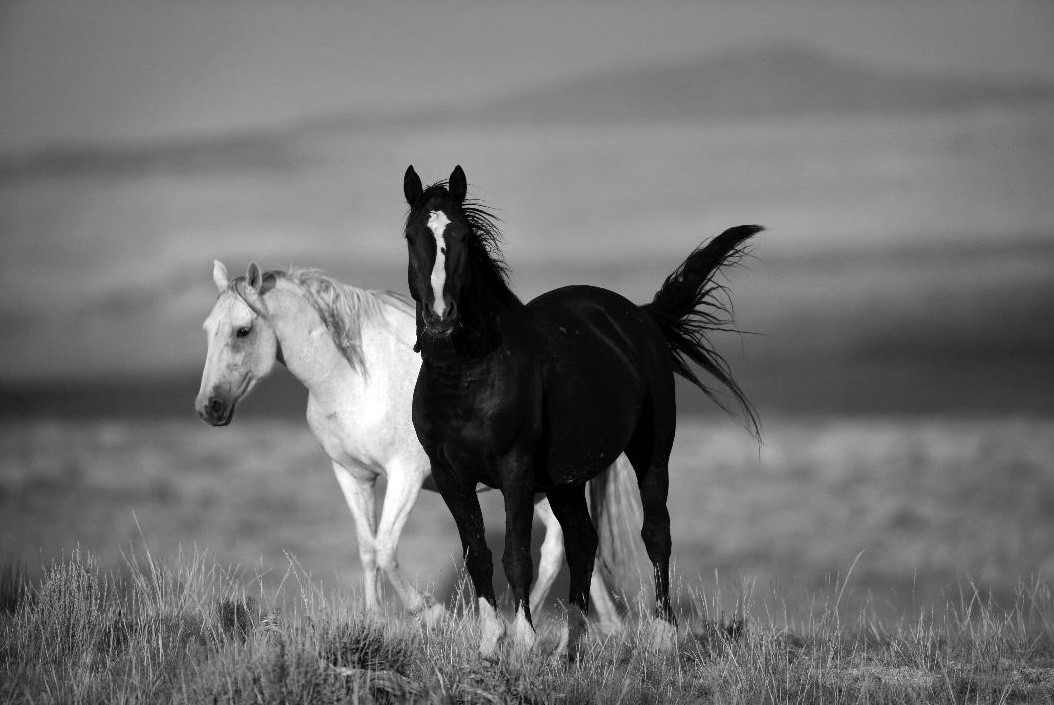
\includegraphics[width = \textwidth]{litreview/imageprocessing/thresholding/horses_grayscale}
      		\caption{Grayscale image. Img: Joe Amon.}
    	\end{subfigure}
    	\begin{subfigure}[b]{0.45\linewidth}
      		\centering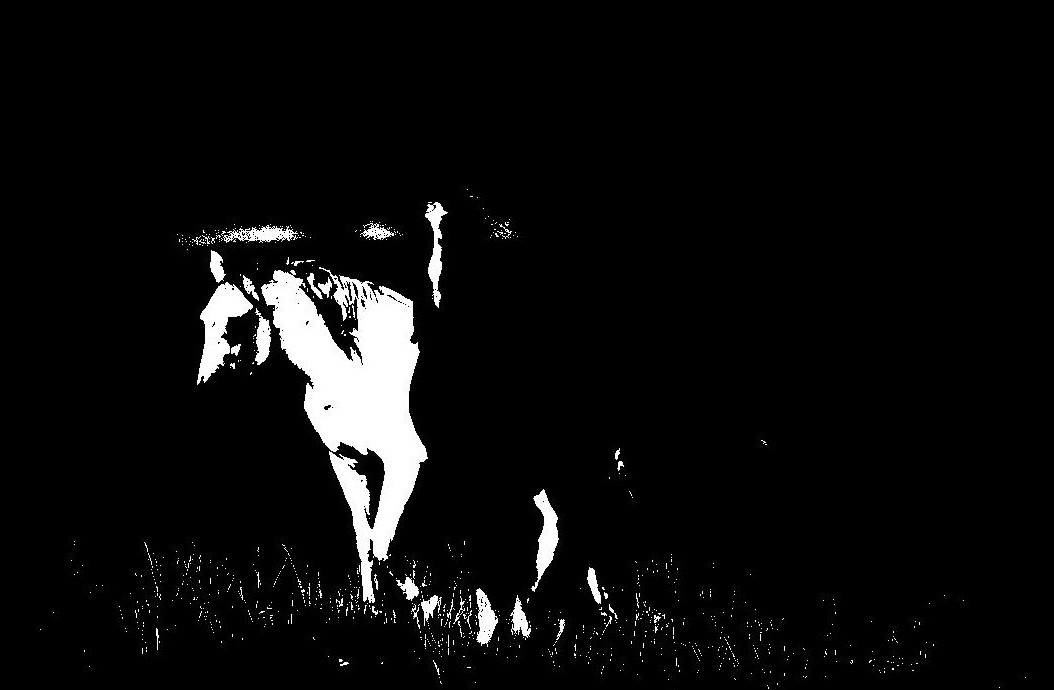
\includegraphics[width = \textwidth]{litreview/imageprocessing/thresholding/horses_binary}
      		\caption{Binary image result of thresholding.}
    	\end{subfigure}
    	\caption{Performing thresholding on a grayscale image to isolate a white horse.}
    	\label{fig:threshex}
\end{figure}

\section{Linear Filtering}

Filtering an image is a way to augment or extract information from it. Linear filtering is a mathematical operation on a neighbourhood of pixels in an image that outputs a weighted average of the pixels in that neighbourhood. It is the weightings of a filter, known as filter coefficients, that determine the effect of the filter. These weights are stored in a matrix called a mask or kernel (see Figure \ref{fig:generalForm}) that's then convolved with an image (see sections \ref{subsection:corr} \& \ref{subsection:conv}).

\begin{figure}[h]
  
   \[ 
     Kernel  = \frac{1}{\sum\limits_{i=0}^{M}\sum\limits_{j=0}^{N}c_{i,j}}
    \begin{bmatrix}
      c_{0,0} & c_{0,1} & \dots & c_{0,n} \\
      c_{1,0} & c_{1,1} & \dots & c_{1,n} \\
      \vdots & \vdots & \ddots & \vdots \\
      c_{m,0} & c_{m,1} & \dots & c_{m,n}
    \end{bmatrix}
  \]
  \caption{General Form of a Linear Filter}
  \label{fig:generalForm}
\end{figure}

% CORRELATION
\subsubsection{Correlation}
\label{subsection:corr}

The correlation of a linear filter $h(u,v)$ to an image $f(i,j)$ with the output $g(i,j)$ may be described mathematically as in Equation \ref{eq:1} but denoted more succinctly as in Equation \ref{eq:correlation_operator}

\begin{equation} \label{eq:1}
g(i,j) = \sum_{u=-k}^{k}\sum_{v = -l}^{l}f(i+u,j+v)h(u,v)
\end{equation}

\begin{equation} \label{eq:correlation_operator}
g = f \otimes h
\end{equation}

Correlation measures the \emph{similarity} between two signals and is used in image processing to measure the similarity between digital images and linear filters. When correlating an image and a linear filter, regions of high similarity will produce high output values \cite{optimalKernel}, this phenomenon can be used to isolate features in an image by correlating a filter that describes the desired feature. A feature could be as simple as a straight line as in a Sobel filter (Figure \ref{fig:sobel_filters}) or as specific as the outline of a car wheel. This method of feature detection is called \emph{template matching} \cite{oreilly_python}. In Figure \ref{fig:sobel_apply} vertical and horizontal Sobel filters \cite{cv_matlab} are correlated with an image a building wall and produce images that emphasize lines that match the orientation of the respective filter. The result is a binary image the output has been thresholded (see section \ref{subsection:thresholding}) to isolate high intensity regions where similarity is greatest.

% SOBEL MASKS
\begin{figure}[H]
  \begin{subfigure}[b]{0.49\textwidth}
    \[k =
    \begin{bmatrix*}[l]
     -1 & -1 & -1 \\
      \phantom{-}2 & \phantom{-}2 & \phantom{-}2 \\
      -1 & -1 & -1 
    \end{bmatrix*}
    \]
    \caption{Horizontal Sobel-Feldman Filter Mask}
    \label{rfidtest_xaxis}
\end{subfigure}
\begin{subfigure}[b]{0.49\textwidth}
  \[ k = 
    \begin{bmatrix}
      -1 & 2 & -1 \\
      -1 & 2 & -1 \\
      -1 & 2 & -1
    \end{bmatrix}
    \]
    \caption{Vertical Sobel-Feldman Filter Mask}  
\end{subfigure}
    \caption{Sobel Filters}
    \label{fig:sobel_filters}
\end{figure}

% SOBEL FILTER APPLICATION
\begin{figure}[H]
  \centering
  \begin{subfigure}[b]{0.3\textwidth}
      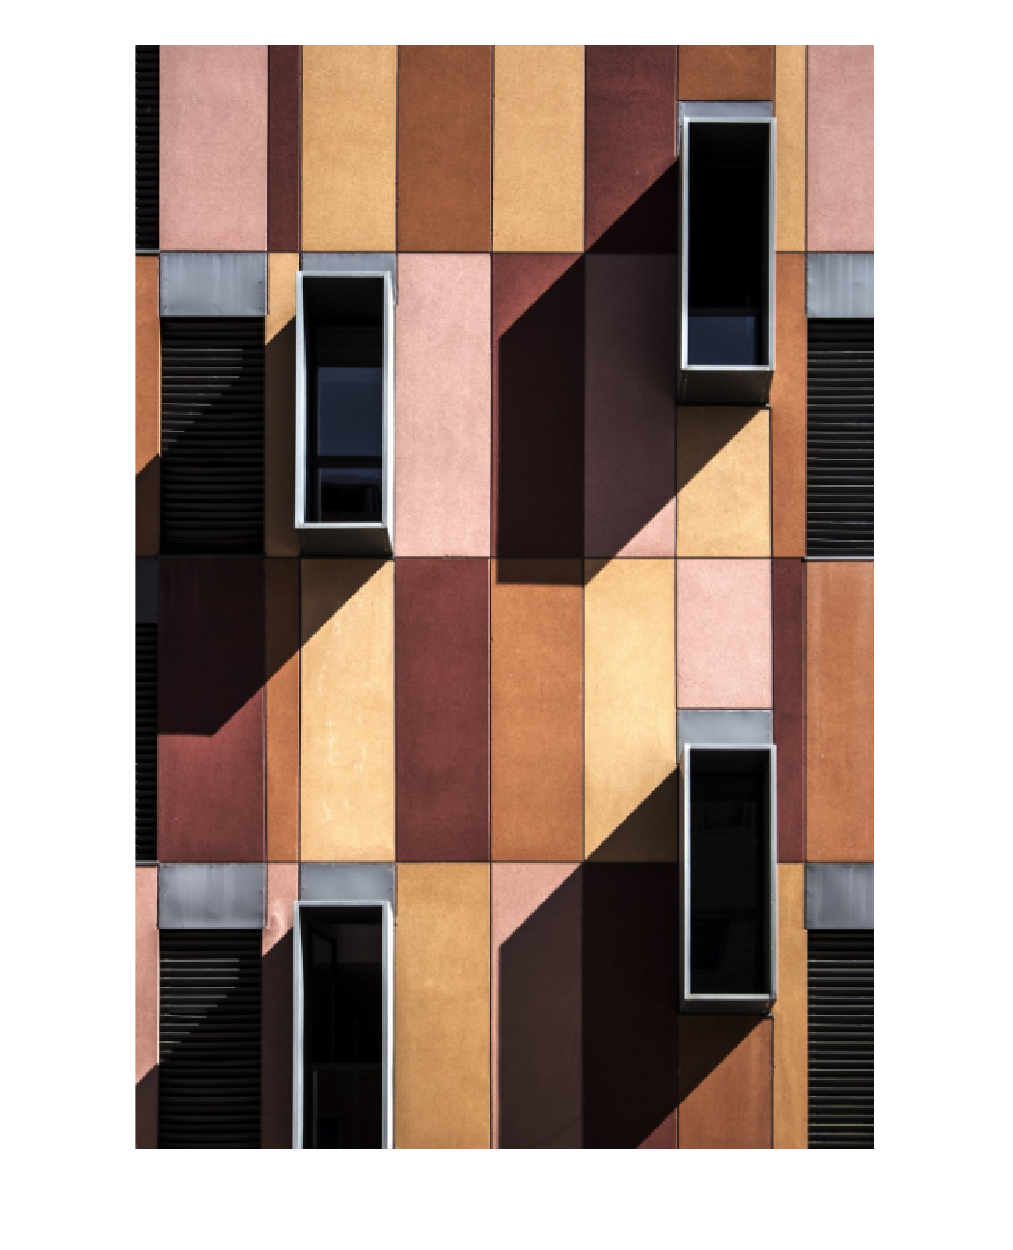
\includegraphics[width=\textwidth]{im_color}
      \caption{Grayscale image. Img: Simone Hutsch}
  \end{subfigure}
  \begin{subfigure}[b]{0.3\textwidth}
      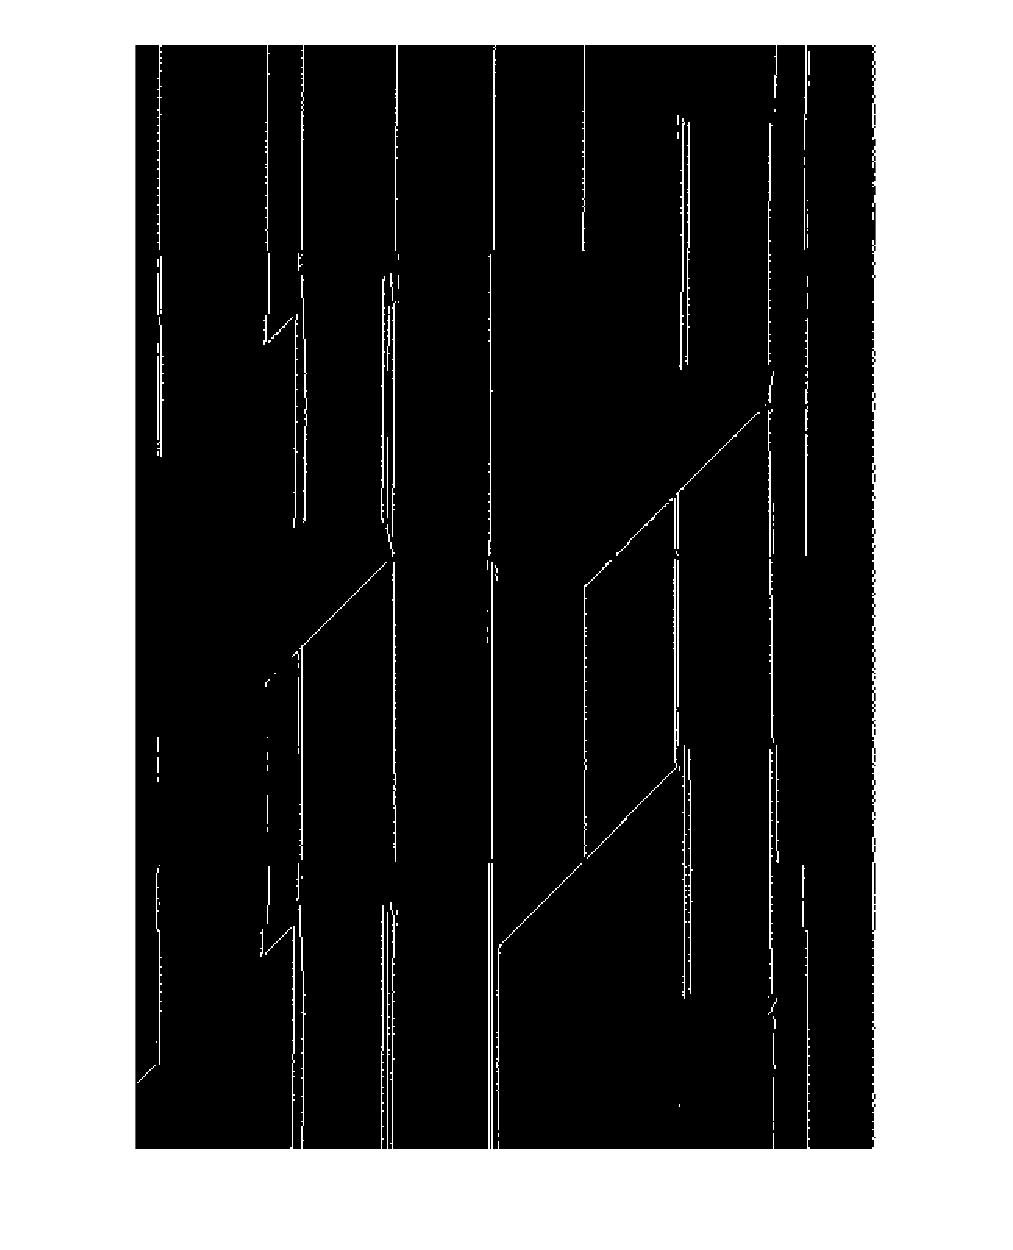
\includegraphics[width=\textwidth]{gv}
      \caption{Binary vertical similarity.}
      \label{fig:vert}
  \end{subfigure}
  \begin{subfigure}[b]{0.3\textwidth}
      
\includegraphics[width=\textwidth]{gh}
      \caption{Binary horizontal similarity.}
      \label{fig:hoz}
  \end{subfigure}
  \caption{Application of Sobel filters to exaggerate lines.}
  \label{fig:sobel_apply}
\end{figure}

Correlation is \emph{shift invariant}, which means that it does the same thing no matter where in an image it is applied. To satisfy this property correlation may be super-positioned 

\[a(f_1 + f_2) = af_1 + af_2\]

and abides by the shift invariance principle

\[g(i,j)=f(i+k,j+l) \Leftrightarrow\ (h\circ g)(i,j)=(h\circ f)(i+k,j+l)\]

Correlation has the side effect of flipping both horizontally and vertically the location of output points relative to the center point (\emph{reference point}) in the original image which may be undesirable as can be observed in Figure \ref{fig:correlation}.

% CORRELATION EXAMPLE  %
\begin{figure}[H] 
  \centering
  \begin{tabular}{ccccc}
      \begin{tabular}{|c|c|c|c|c|}
      \hline
      0 & 0 & 0 & 0 & 0 \\[1pt]
      \hline
      0 & 0 & 0 & 0 & 0 \\[1pt]
      \hline
      0 & 0 & 1 & 0 & 0 \\[1pt]
      \hline
      0 & 0 & 0 & 0 & 0 \\[1pt]
      \hline
      0 & 0 & 0 & 0 & 0 \\[1pt]
      \hline
      \end{tabular}%
    & $\otimes$ &
    \begin{tabular}{|c|c|c|}
      \hline
      a & b & c \\
      \hline
      d & e & f \\
      \hline
      g & h & i \\
      \hline 
    \end{tabular}
    & $=$ &
    \begin{tabular}{|c|c|c|c|c|}
      \hline
      0 & 0 & 0 & 0 & 0 \\[1pt]
      \hline
      0 & \textbf{i} & \textbf{h} & \textbf{g} & 0 \\[1pt]
      \hline
      0 & \textbf{f} & \textbf{e} & \textbf{d} & 0 \\[1pt]
      \hline
      0 & \textbf{c} & \textbf{b} & \textbf{a} & 0 \\[1pt]
      \hline
      0 & 0 & 0 & 0 & 0 \\[1pt]
      \hline
    \end{tabular} \\
    $F(x,y)$ & & $H(u,v)$& & $G(x,y)$ \\
  \end{tabular}
  \caption{Correlation of a filter and an image.}
  \label{fig:correlation}
\end{figure}
\subsection{Convolution}
\label{subsection:conv}
Convolution is also a linear operation that is shift invariant. It is very similar to correlation except that where correlation measure similarity between signals convolution measures the effect of one signal on another. It is described mathematically by the expression,

\[ g(i,j) = \sum_{u=-k}^{k}\sum_{v = -l}^{l}f(u,v)h(i-u,j-v)\]

Notice that the filter $h(i,j)$ is rotated  180 degrees. This causes the output's orientation to match the original image. Convolution may be notated as follows,

\[g = f \ast h\]

Convolution is essentially the same as correlation except that it doesn't flip the output relative to the original image as can be seen in Figure \ref{fig:convolution} and it is the operation that is performed when a linear filter is applied to a digital image.

% Convolution example  %
\begin{figure}[H] 
  \centering
  \begin{tabular}{ccccc}
      \begin{tabular}{|c|c|c|c|c|}
      \hline
      0 & 0 & 0 & 0 & 0 \\[1pt]
      \hline
      0 & 0 & 0 & 0 & 0 \\[1pt]
      \hline
      0 & 0 & 1 & 0 & 0 \\[1pt]
      \hline
      0 & 0 & 0 & 0 & 0 \\[1pt]
      \hline
      0 & 0 & 0 & 0 & 0 \\[1pt]
      \hline
      \end{tabular}%
    & $\ast$ &
    \begin{tabular}{|c|c|c|}
      \hline
      a & b & c \\
      \hline
      d & e & f \\
      \hline
      g & h & i \\
      \hline 
    \end{tabular}
    & $=$ &
    \begin{tabular}{|c|c|c|c|c|}
      \hline
      0 & 0 & 0 & 0 & 0 \\[1pt]
      \hline
      0 &  \textbf{a} & \textbf{b} & \textbf{c} & 0 \\[1pt]
      \hline
      0 & \textbf{d} & \textbf{e} & \textbf{f} & 0 \\[1pt]
      \hline
      0 & \textbf{g} & \textbf{h} & \textbf{i} & 0 \\[1pt]
      \hline
      0 & 0 & 0 & 0 & 0 \\[1pt]
      \hline
    \end{tabular} \\
    $F(x,y)$ & & $H(u,v)$& & $G(x,y)$ \\
  \end{tabular}
  \caption{Convolution of a filter and an image.}
  \label{fig:convolution}
\end{figure}
\subsection{Kernels}

Kernels are just the weightings that define the characteristics of a filter, also known as a filter's mask. A filter kernel is nearly always square so as to have a center cell which sits atop a reference pixel. The result of the filter's application at that reference pixel will be stored in the output image at the location of the reference pixel. Notice in Figure \ref{fig:kernel_graphics} how the mask sits over the reference pixel.

% TREE %
\begin{figure}[H]
 \centering
 \centering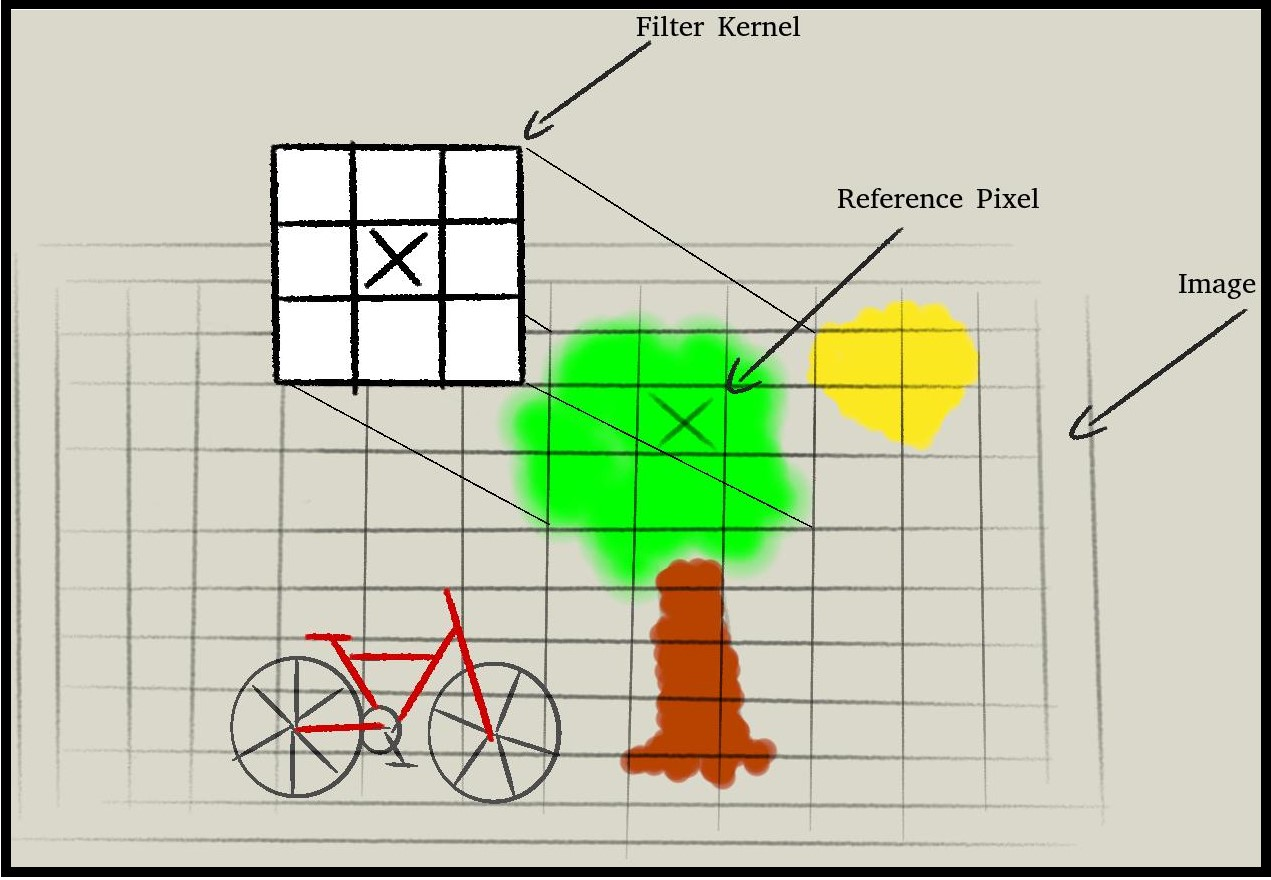
\includegraphics[width=350pt]{kernel_graphics}
 \caption{Visualization of a Filter Kernel Application}
 \label{fig:kernel_graphics}
\end{figure}

\subsubsection{Box Filter}
\label{subsubsection:boxfilter}
A box filter also known as a moving average filter simply outputs the average of its inputs because the filter weights are evenly distributed. By passing this filter over an image its sharpness is reduced giving a smoothing or blurring effect which can sometime be useful in image processing for filtering out noise. This can be observed in Figure \ref{fig:roughDog}.

% DOG BOX FILTERED%
\begin{figure}[H]
 \centering
 \begin{subfigure}[b]{0.75\textwidth}
   \centering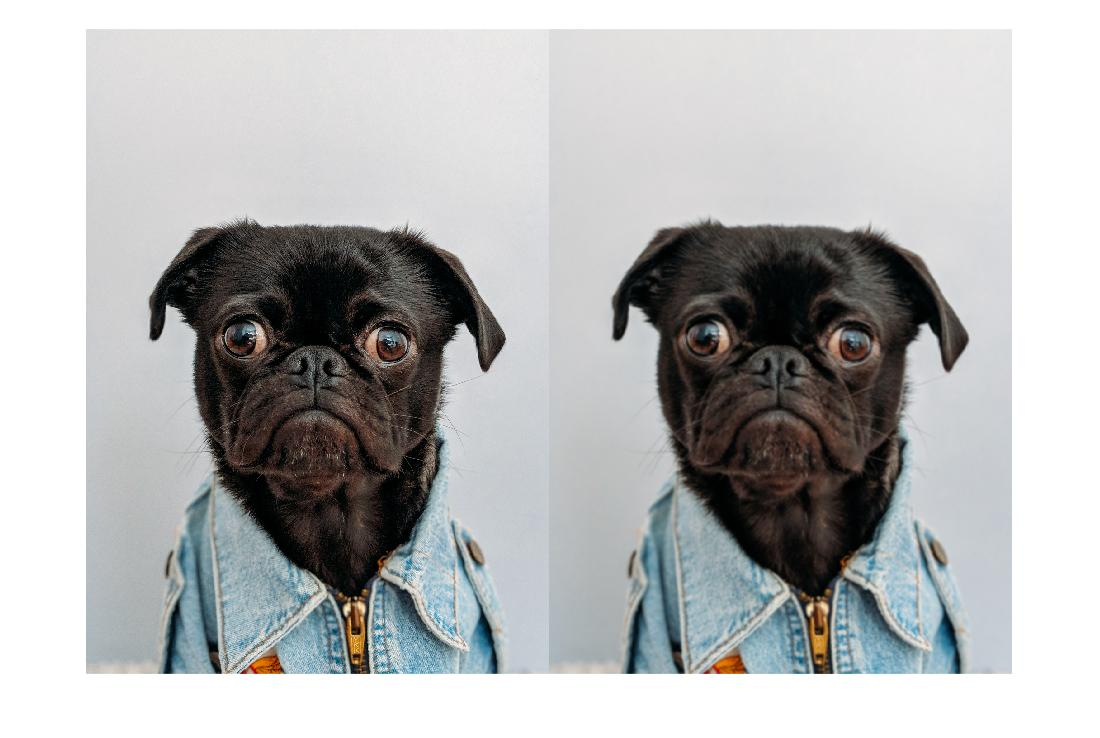
\includegraphics[width=300pt]{dogPug}
   \caption{Left: Photo by Charles Deluvio. Right: Application of $16\times16$ box filter.}
   \label{fig:roughDog}
 \end{subfigure}
 \begin{subfigure}[b]{0.25\textwidth}
   \centering
   \[
     \frac{1}{9}
   \begin{bmatrix}
      1 & 1 & 1 \\
      1 & 1 & 1 \\
      1 & 1 & 1
   \end{bmatrix}
   \]
   \caption{Box Filter Kernel.}
   \label{fig:boxkernel}
 \end{subfigure}
 \caption{Box Filter application and kernel.}
 \label{fig:boxfilter}
\end{figure}

\subsubsection{Gaussian Kernel}

The Gaussian is a rather important kernel in image processing as it models the Gaussian function (see Section \ref{section:gaussian}) or normal distribution. This filter is perhaps most well known for filtering noise but retaining edge sharpness better than other denoising filters. It works in a similar fashion to the moving average filter but as you can see in Figure XXX it is superior at filtering out the noise in comparison as it retains better edge definition. The reason the Gaussian filter is superior is because it addresses two properties about images that a generally true, 
\begin{enumerate}
    \item The actual value of a pixel is probably the same or similar to its neighbors. 
    \item Each pixel of noise in an image is added independently.
\end{enumerate}

The Gaussian which models the Normal distribution addresses both of these qualities by having high value cooefficients at the filter's center and lower values tapering out to the edges of the filter. Which essentially means values closer together are more strongly correlated than those further away from the reference pixel as can be observed in the 16x16 Gaussian filter kernel in Figure XXX.

[ Add Denoising using Gaussian Example ]
[ Add matrix of kernel filter. ]







\subsection{Nonlinear Filtering}

Non-linear filtering refers to a set of operations that, like linear filters, are performed on a neighborhood of pixels in a digital image and have a filter kernel that defines the filter's behaviour. Unlike linear filters, the application of nonlinear filters is not linearly shift invariant, however there are scenarios where a non-linear filter can achieve unique or superior results to linear filters. A non-linear filter's application to an image is not simply it's convolution with that image but will follow a an filter specific algorithm. 

This section of the report details some of the nonlinear filters relevant to the reports subject matter.



\subsubsection{The Median Filter}
\label{subsubsection:median_filter}

The median filter is useful for denoising an image, much like the linear box filter and Gaussian filters (section \ref{subsubsection:kernels}). A median filter returns the median value of the pixel found in the application neighbourhood. This is a more complex operation than to convolve one signal with another however it can be computed in linear time \cite{cormen_2001}. It is often superior to the Gaussian filter at denoising images because it preserves edges and is not influenced by outlier intensities unlike a linear filter. In Figure \ref{fig:shot_noise} the median filter demonstrates a superior ability to remove salt and pepper noise as compared to the Gaussian filter.

\begin{figure*}[htbp]
    \centering 
    \begin{subfigure}[b]{0.3\textwidth}
        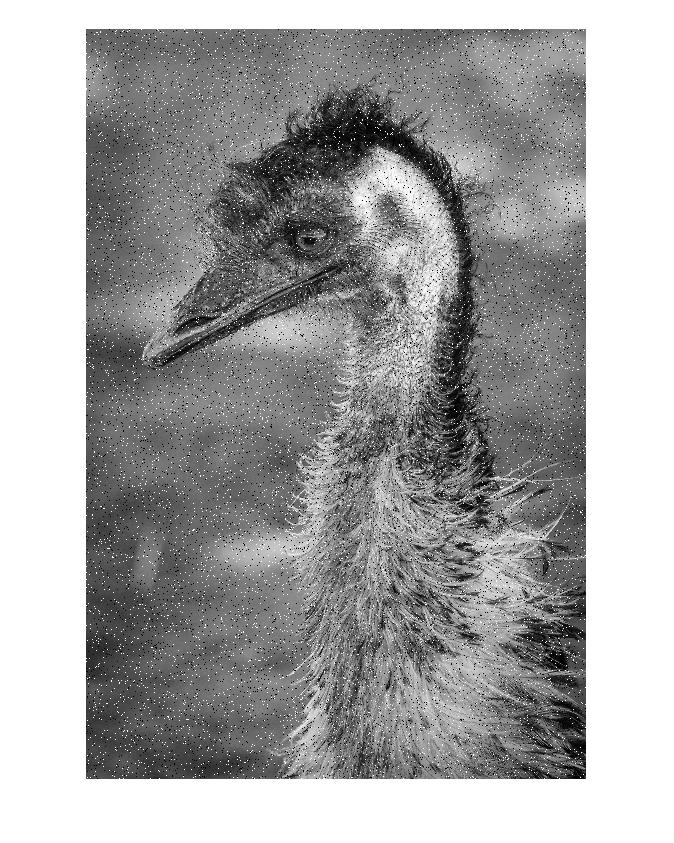
\includegraphics[width=\textwidth]{emu_noise}
        \caption{Salt and Pepper Noise}
        \label{fig:emu_noise}
    \end{subfigure}
    \begin{subfigure}[b]{0.3\textwidth}
        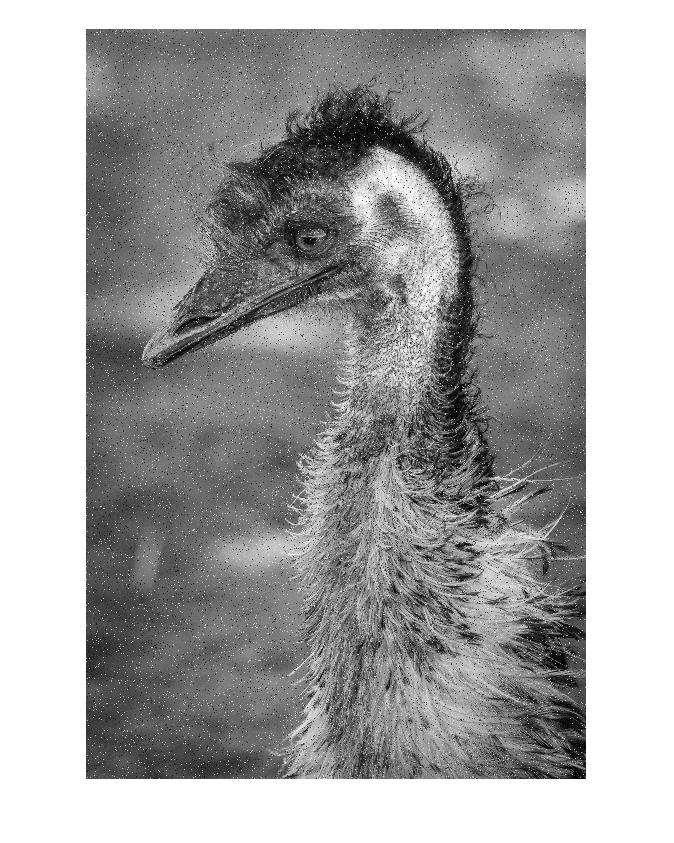
\includegraphics[width=\textwidth]{emu_gauss}
        \caption{7x7 Gaussian}
        \label{fig:emu_gauss}
    \end{subfigure}
    \begin{subfigure}[b]{0.3\textwidth}
        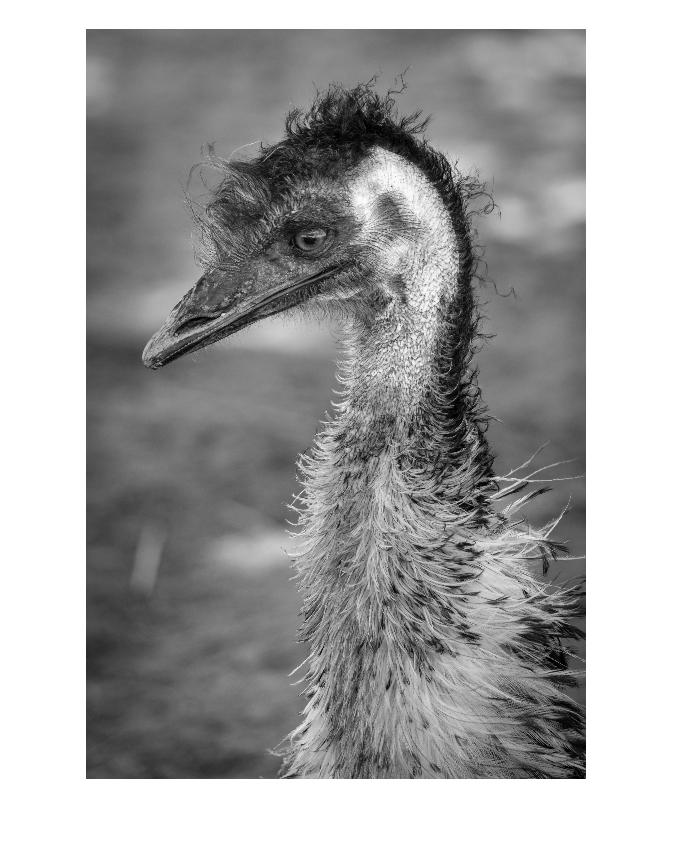
\includegraphics[width=\textwidth]{emu_median}
        \caption{7x7 Median Filter}
        \label{fig:emu_median}
    \end{subfigure}
    \captionsetup{format=hang}
    \caption{Filtering out salt and pepper noise with Gaussian and median filter. Original image by Grant Durr.}
    \label{fig:shot_noise}
\end{figure*}

Huang's Algorithm \ref{algorithm:median_filter} is one possible implementation \cite{median_filter_new}\cite{median_filter_3} of a median filter for a 2D image and is simple and of linear computational complexity, O(n). In this algorithm the histogram $H$ refers to the neighbourhood under the filter's mask. Each time the filter is moved the the histogram's leftmost column is removed and the rightmost column is added. The median is calculated for the first window position thereafter a count of the number of picture elements (pels) in a window having a value less than the current window's median is maintained. If more than half of the window's pels have a value are less than the last window's median then the median value is reduced until the number of pels with a value less than the median is greater than or equal to half of the total window pels, in this way the median value is selected. Finally the median is stored in the output image $Y$ at location $(i,j)$. 

\begin{algorithm}[H]
    \SetAlgoLined
    \KwInput{Image X of size MxN, filter size n} 
    \KwOutput{Image Y of the same size as X}
    Initialize histogram H\;
    \For{i = 1 to M}
    {
        \For{j = 1 to N}
        {
            % \For{k = $\frac{-n}{2}$ to $\frac{n}{2}$}
            \For{$k = \frac{-n}{2}$ to $\frac{n}{2}$}
            {
                Remove $X_{i+k,j-\frac{n}{2}-1}$  from H\;
                Add $X_{i+k,j+\frac{n}{2}}$ to H\; 
            }
            $Y_{i,j} \leftarrow median(H,k)$\;
        }
    }
\caption{Huang's Median Filtering Algorithm \cite{median_filter_old}}
\label{algorithm:median_filter}
\end{algorithm}
\subsubsection{Morphology}
\label{subsubsection:morphology}
Morphological operators are a set of neighborhood operators that modify the shape of objects in binary images. A binary image is most often produced by thresholding (see section \ref{subsection:thresholding}) a grayscale image, Figure \ref{fig:thresholding} shows the conversion of an RGB image to a binary one, here the white pixels are regarded as objects sometimes referred to as 'blobs'.Morphological operations are used if you wish to modify blobs, for example to change total area of blob and to connect or separate two or more blobs. Morphological operators, like filters, depend on a kernel that characterises their behaviour which is called a \emph{structuring element}. There are two fundamental morphological operations, \emph{dilation} and \emph{erosion}, that all others are a combination of \cite{morph_textbook}. 

\begin{figure}[htbp]
    \centering
    \begin{subfigure}[b]{0.3\textwidth}
        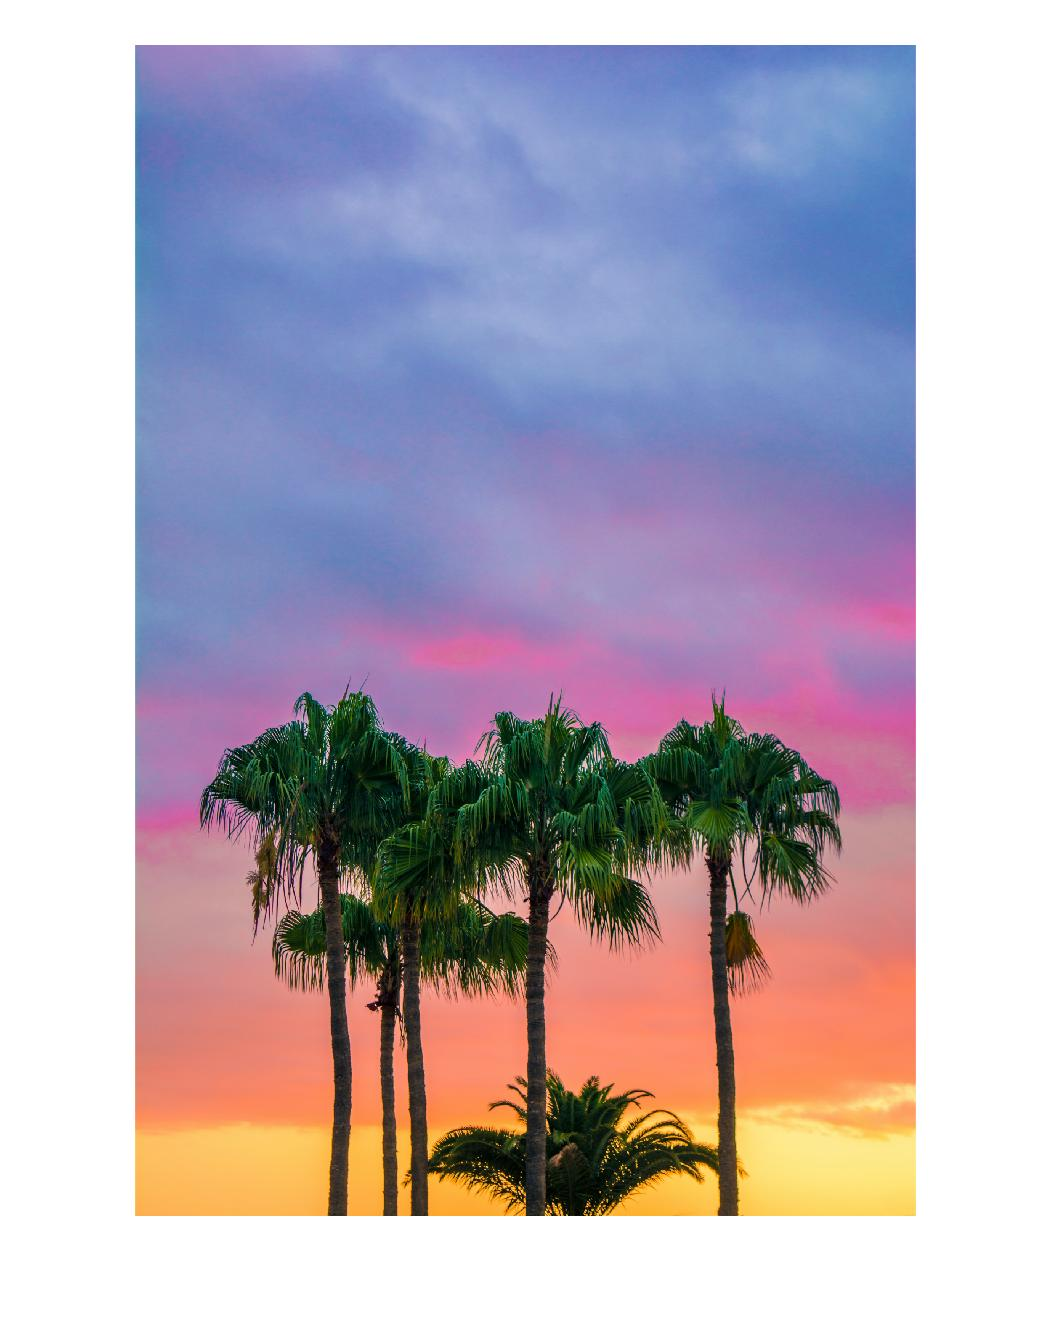
\includegraphics[width=\textwidth]{palms_resized}
        \caption{RGB Image}
        \label{fig:emu_noise}
    \end{subfigure}
    \begin{subfigure}[b]{0.3\textwidth}
        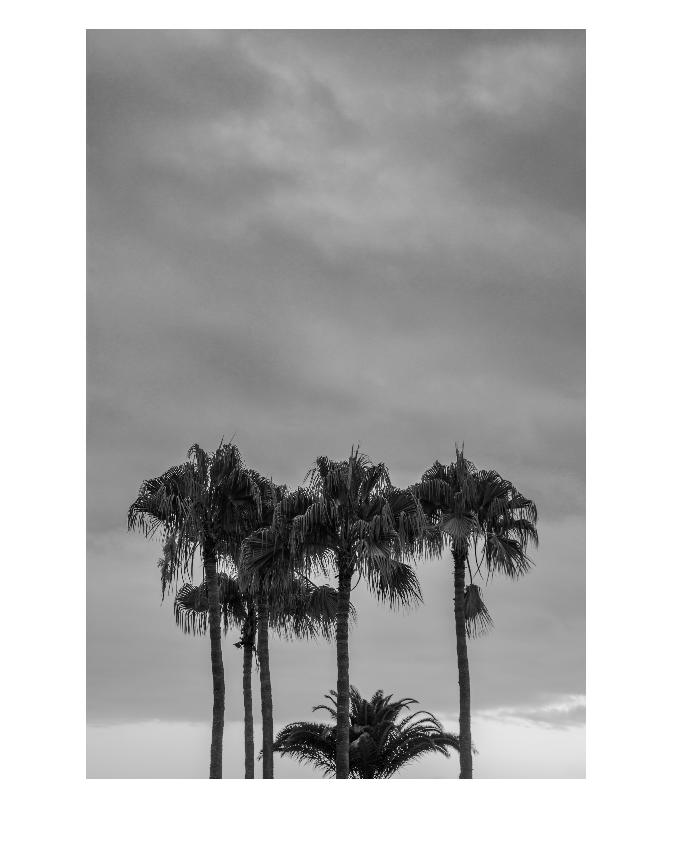
\includegraphics[width=\textwidth]{palms_grayscale}
        \caption{Grayscale Conversion}
        \label{fig:emu_gauss}
    \end{subfigure}
    \begin{subfigure}[b]{0.3\textwidth}
        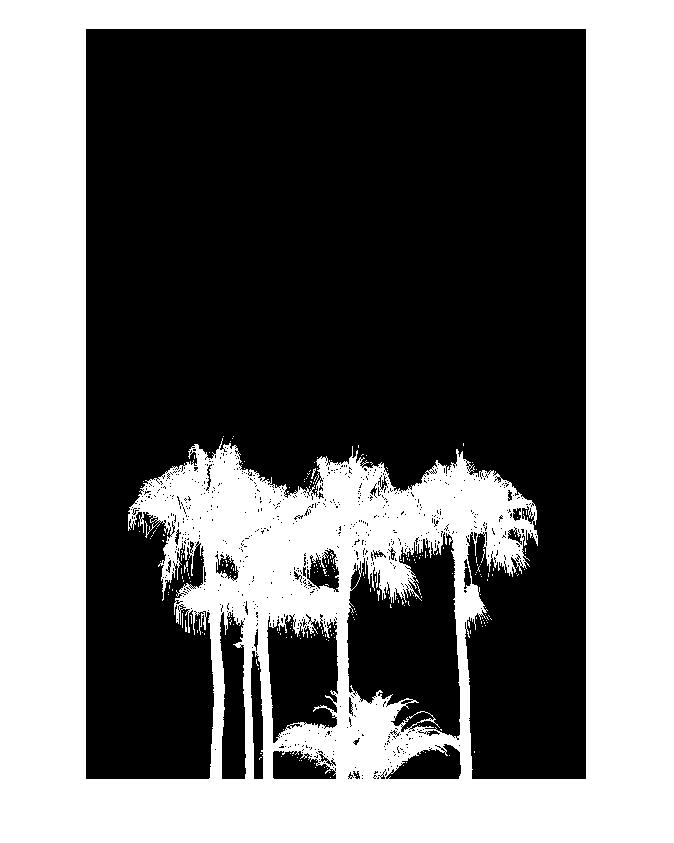
\includegraphics[width=\textwidth]{palms_binary}
        \caption{Binary Thresholding}
        \label{fig:emu_median}
    \end{subfigure}
    \captionsetup{format = hang}
    \caption{Conversion of an RGB image to a binary image. Original image by Adam Birkett}
    \label{fig:thresholding}
\end{figure}

\subsubsection{Structuring Elements}

A 2D structuring element itself is a matrix of binary values, generally a smaller than the image it's to operate on, and is of a similar function to a filter kernel, as it largely characterises the effect of the morphological operation it's being used for. A structuring element has a reference pixel or origin that determines where the result of the morphological operation is stored in the output image. Structuring element shapes are selected according to the scenario it's to be used in, for example if you want to produce round edges on blobs you might use a disc structuring element and if you want to produce straight edges you would use a rectangular structing element. Figure \ref{fig:structuring_elements} shows some example shape and size structuring elements. Structuring elements must always have odd dimensions so as to have a centred origin at which to store the output.

\begin{figure}[htbp]
    \centering
    \begin{subfigure}[b]{0.3\textwidth}
           \[ \begin{bmatrix}
                1 & 1 & 1 & 1 & 1\\
                1 & 1 & 1 & 1 & 1\\
                1 & 1 & 1 & 1 & 1\\
                1 & 1 & 1 & 1 & 1\\
                1 & 1 & 1 & 1 & 1\\
             \end{bmatrix}\]
        \captionsetup{format = hang}
        \caption{5x5 Rectangular Structuring Element}
    \end{subfigure}
    \begin{subfigure}[b]{0.3\textwidth}
        \[\begin{bmatrix}
            0 & 0 & 1 & 0 & 0\\
            0 & 1 & 1 & 1 & 0\\
            1 & 1 & 1 & 1 & 1\\
            0 & 1 & 1 & 1 & 0\\
            0 & 0 & 1 & 0 & 0\\
         \end{bmatrix}\]
        \captionsetup{format = hang}
        \caption{5x5 Diamond Structuring Element}
    \end{subfigure} 
    \begin{subfigure}[b]{0.3\textwidth}
       \[\begin{bmatrix}
            0 & 0 & 1 & 0 & 0\\
            0 & 0 & 1 & 0 & 0\\
            1 & 1 & 1 & 1 & 1\\
            0 & 0 & 1 & 0 & 0\\
            0 & 0 & 1 & 0 & 0\\
         \end{bmatrix}\]
        \captionsetup{format = hang}
        \caption{5x5 Cross Structuring Element}
    \end{subfigure}
    \captionsetup{format = hang}
    \caption{}
    \label{fig:structuring_elements}
\end{figure}


\subsubsection{Performing a morphological operation}

A morphological operation is performed by first convolving a structuring element with a neighbourhood of an image and then thresholding the result. The threshold level determines the type of operation that is performed \cite{alg_apps}. Algorithm \ref{algorithm:morphological_operation} outlines how a morphological operation can be implemented.

\begin{algorithm}
\SetAlgoLined
\KwIn{Binary Image X of size MxN}
\KwOut{Binary Image Y of size MxN}
Initialize: structuring element se, threshold level T\;
\For{i = 0 to M}
{
    \For{j = 0 to N}
    {
        convolutionSum = se $\ast$ neighborhoodCentered(X[i,j])\;
        \eIf{convolutionSum $\geq$ T}{
            Y[i,j] = 1\;
        }{
            Y[i,j] = 0\;
        }
    }
}
\caption{Performing a morphological operation.}
\label{algorithm:morphological_operation}
\end{algorithm}

\subsubsection{Fundamental Morphological Operations}

\textbf{Dilation} inflates the size of a blob, the scale and nature of the inflation is determined by the size and shape of specific structuring element used for the operation. In Figure \ref{fig:ice_dilation} a square structuring element is used to fill gaps between objects and for their size to increase, this can be useful in situations where we want to combine blobs that are close together but have small gaps between them. In \ref{algorithm:morphological_operation} to specify that we want a dilation to be performed the threshold value should be set to 1. This means that if a single cell of the structuring element shape is touching a blob the output of the operation will be a 1, increasing the size of the blob in that neighbourhood. 

\textbf{Erosion} performs the opposite function to dilation by causing objects to contract rather than grow. To specify an erosion operation the threshold value in Algorithm \ref{algorithm:morphological_operation} should be set to the sum of the elements in the structuring element. This means that for the output of an erosion operation to be 1 the entire structuring element has to be inside of a blob, anywhere the structuring element overlaps black background the blob will be eroded. In Figure \ref{fig:ice_erosion} many smaller entities are erased from the image and blob edges are smoothed. Erosion can be used to clean up small noise-like blobs from binary images but will also modify blobs that are not regarded as noise-like, by shrinking them and smoothing their edges.

\textbf{Opening} is a composite operation comprised of an erosion and then dilation, the same or different structuring element may be used for each. The effect of this order of operations is to first clear away small blobs and increase the smoothness of and separation between existing blobs and then to consolidate the the remaining blobs by performing a dilation. This is a useful operation if you want to join together blobs that are close together but not touching but first remove any noise-like blobs so that they don't become enlarged. Figure \ref{ref:ice_open} shows the effect of opening with a square structuring element, notice that the small blobs are cleared away but the remaining objects are thickened and most original blobs separation is preserved. 

\textbf{Closing} is the dual of opening and performs first a dilation and then an erosion. This order of operations is useful if you wish to consolidate blobs into large single entities before performing an erosion that clean them up and remove any remaining blobs. Figure \ref{fig:ice_close} shows how a closing was able to remove small noise-like entities but preserve and join larger blobs.

\renewcommand{\arraystretch}{0.6} % because \baselinestretch is 1.6667
\begin{figure}[H]
    \centering
    \begin{subfigure}[b]{0.49\textwidth}
        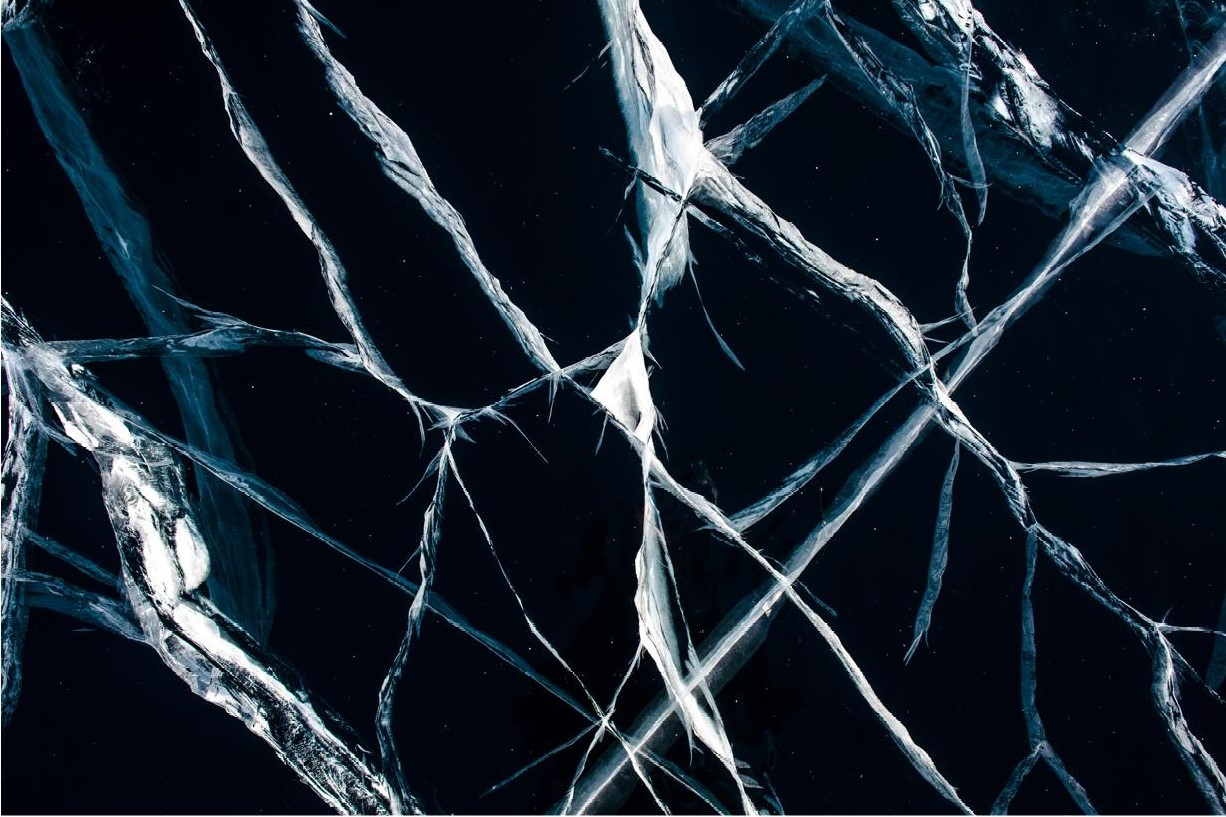
\includegraphics[width=\textwidth]{litreview/imageprocessing/nonlinear/morphology/ice_original}
        \caption{Img: Daniel Born}
        \label{fig:ice}
    \end{subfigure}
    \begin{subfigure}[b]{0.49\textwidth}
        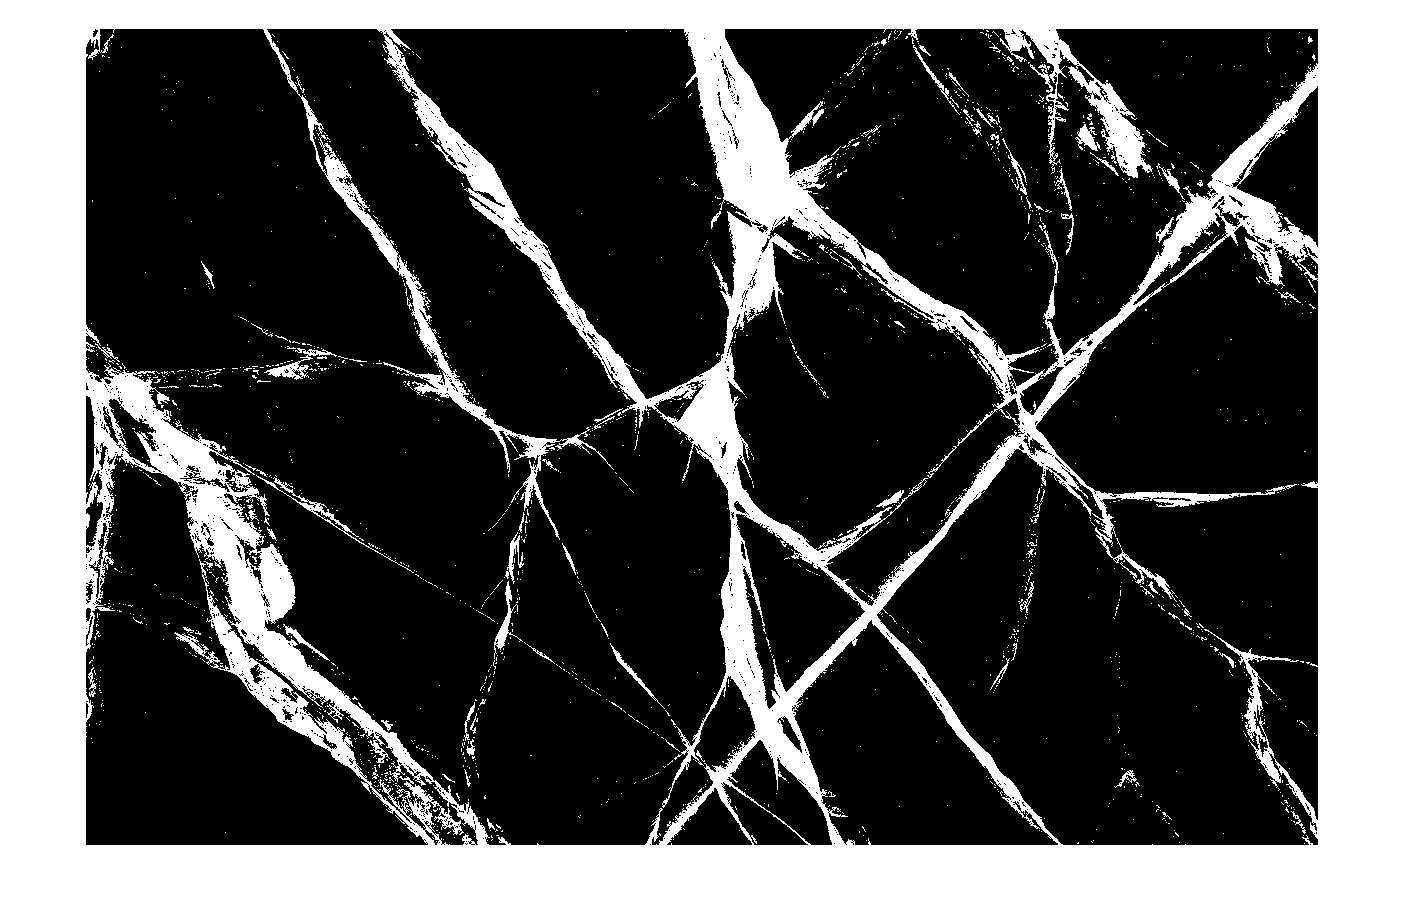
\includegraphics[width=\textwidth]{litreview/imageprocessing/nonlinear/morphology/ice_binary}
        \caption{Binarized image}
        \label{fig:ice_binary}
    \end{subfigure}
    \begin{subfigure}[b]{0.49\textwidth}
        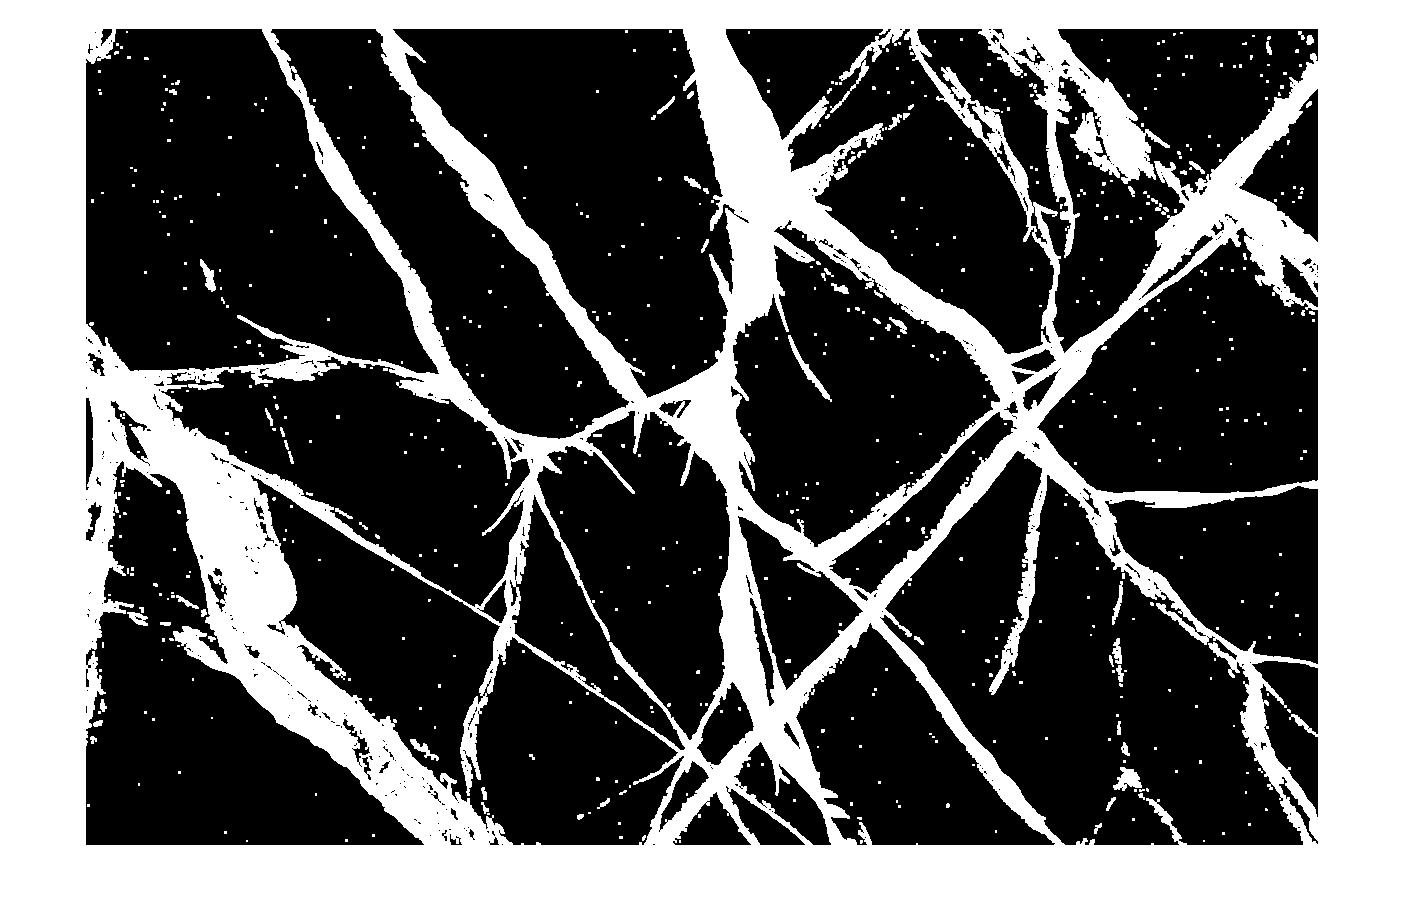
\includegraphics[width=\textwidth]{litreview/imageprocessing/nonlinear/morphology/ice_dilate}
        \caption{Dilation}
        \label{fig:ice_dilation}
    \end{subfigure}
    \begin{subfigure}[b]{0.49\textwidth}
        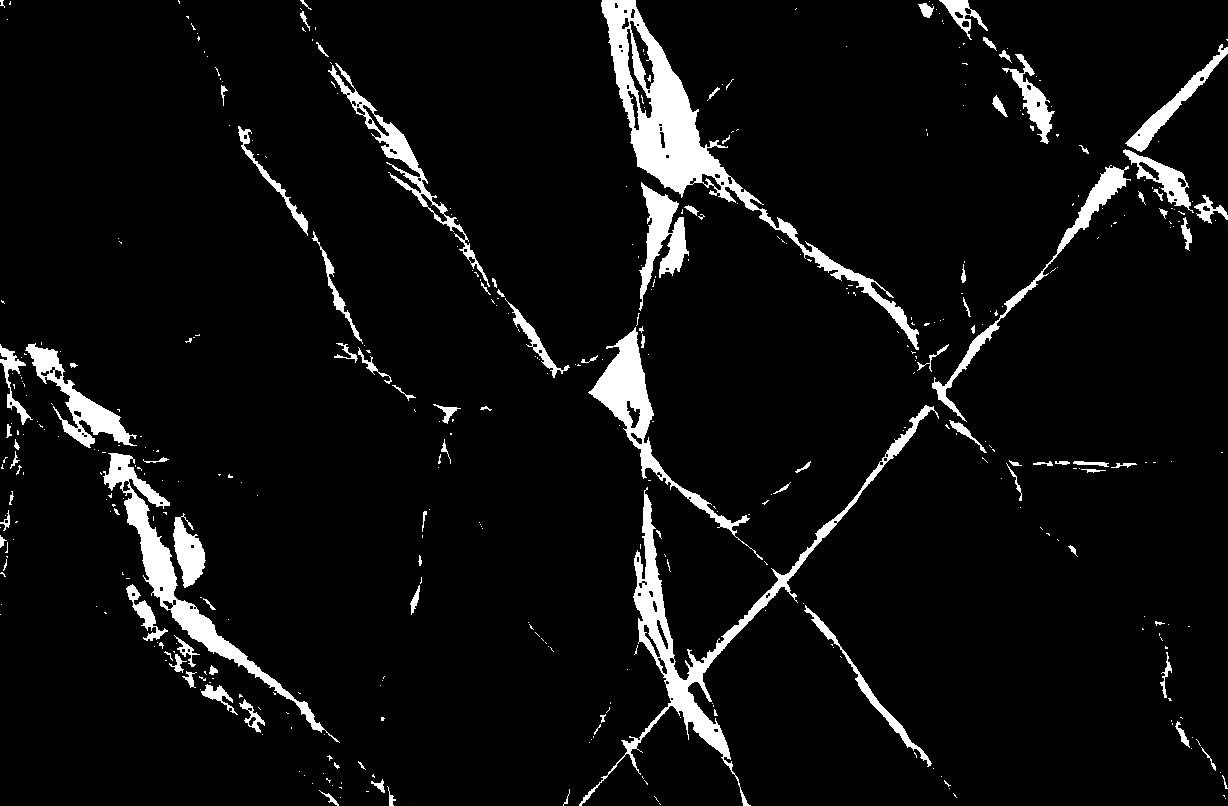
\includegraphics[width=\textwidth]{litreview/imageprocessing/nonlinear/morphology/ice_erode}
        \caption{Erosion}
        \label{fig:ice_erosion}
    \end{subfigure}
    \begin{subfigure}[b]{0.49\textwidth}
        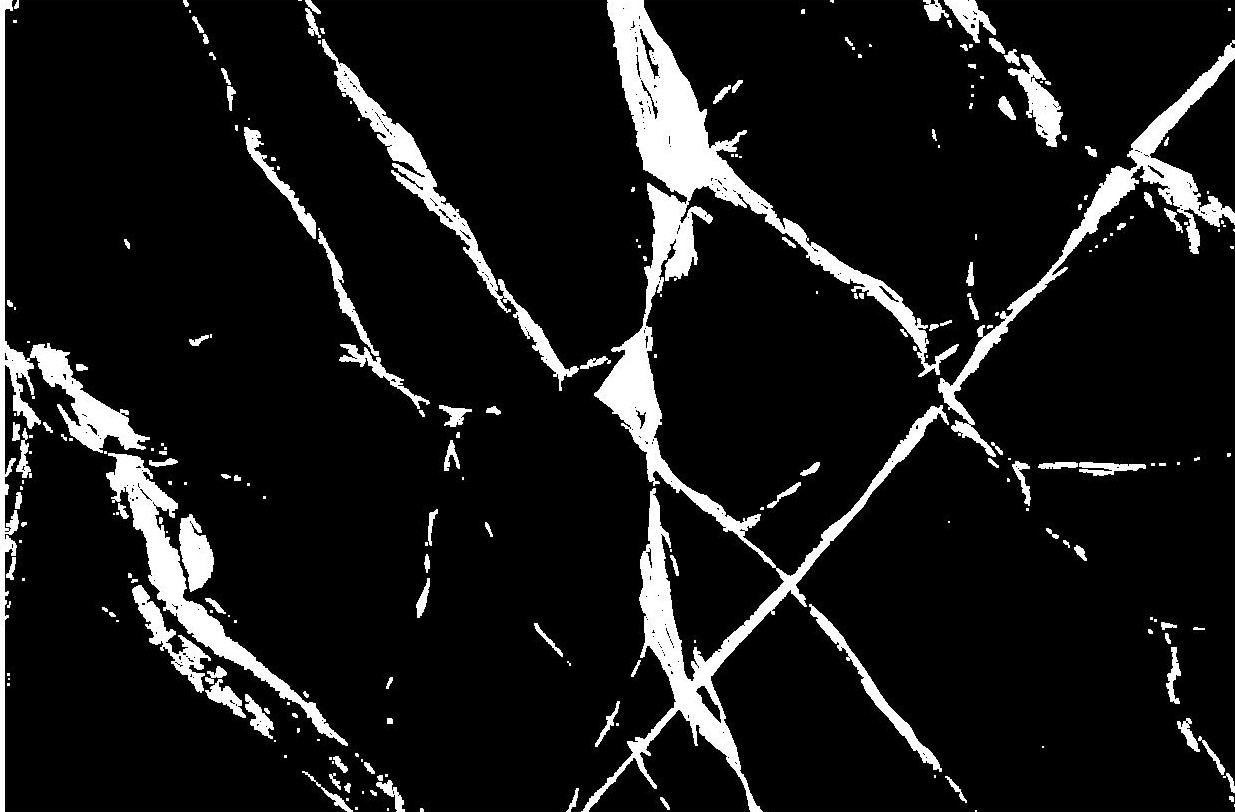
\includegraphics[width=\textwidth]{litreview/imageprocessing/nonlinear/morphology/ice_open}
        \caption{Opening}
        \label{fig:ice_open}
    \end{subfigure} 
    \begin{subfigure}[b]{0.49\textwidth}
        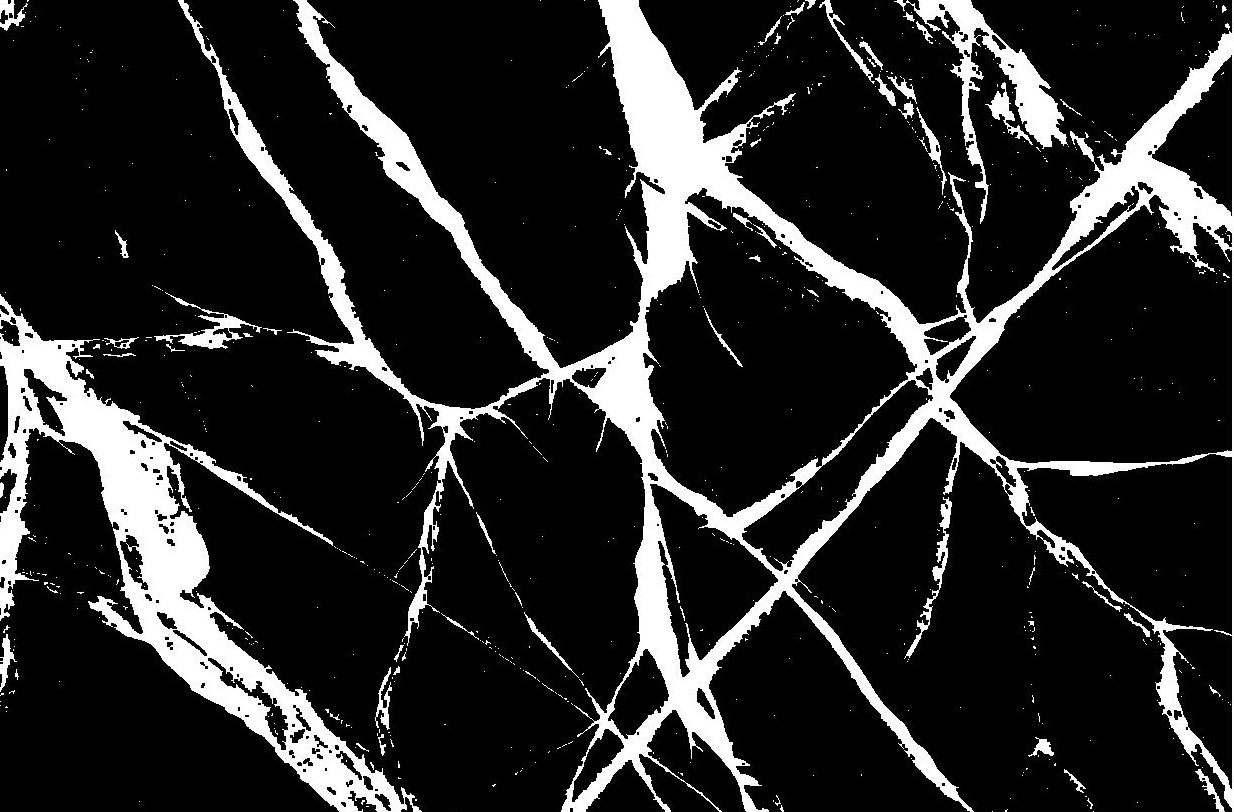
\includegraphics[width=\textwidth]{litreview/imageprocessing/nonlinear/morphology/ice_close}
        \caption{Closing}
        \label{fig:ice_close}
    \end{subfigure} 
    \captionsetup{format = hang}
    \caption{Fundamental morphological  operations performed on a binary image using a 9x9 square structuring element.}
    \label{fig:morphology}
  \end{figure}


